\begin{figure}[ht]
    \centering
    \begin{subfigure}{0.32\textwidth}
        \centering
        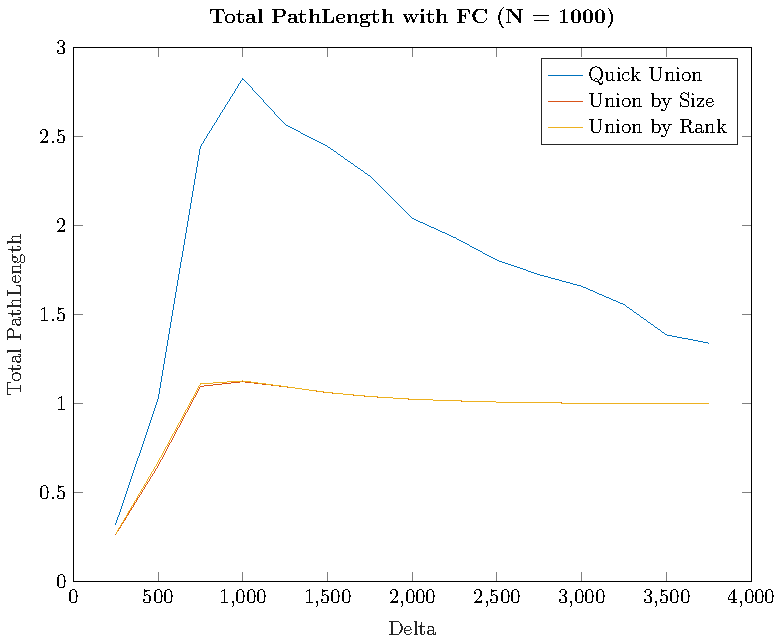
\includegraphics[width=\textwidth]{../images/plotFCFull1000_PathLength.pdf}
        \caption{Path Lengths with different union strategies with $n = 1000$ using Full Compression}
    \end{subfigure}%
    \hfill
    % Subfigure 2
    \begin{subfigure}{0.32\textwidth}
        \centering
        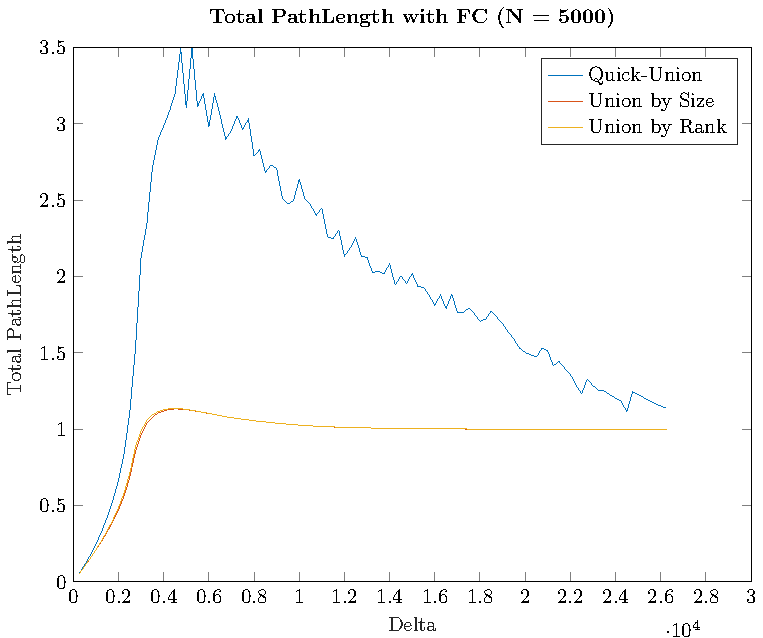
\includegraphics[width=\textwidth]{../images/plotFCFull5000_PathLength.pdf}
        \caption{Path Lengths with different union strategies with $n = 5000$ using Full Compression}
    \end{subfigure}%
    \hfill
    % Subfigure 3
    \begin{subfigure}{0.32\textwidth}
        \centering
        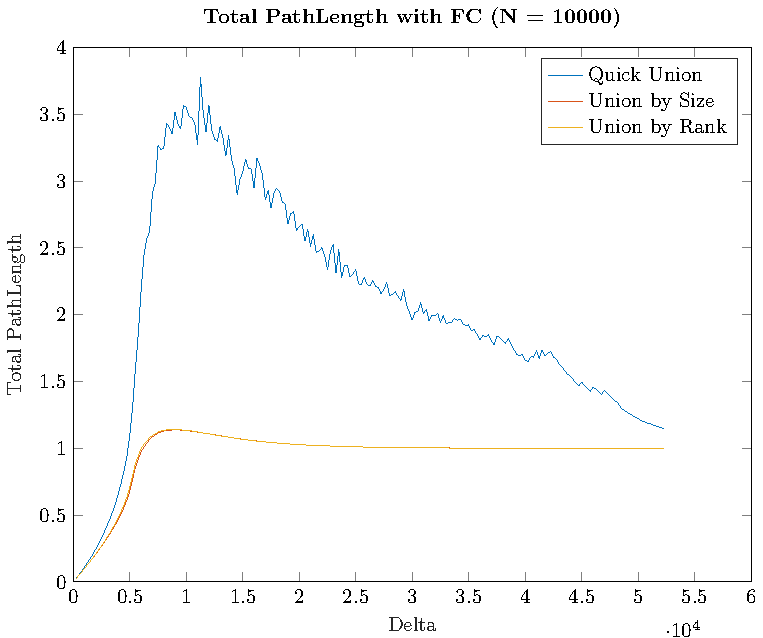
\includegraphics[width=\textwidth]{../images/plotFCFull10000_PathLength.pdf}
        \caption{Path Lengths with different union strategies with $n = 10000$ using Full Compression}
    \end{subfigure}
    % Subfigure 1
    \begin{subfigure}{0.32\textwidth}
        \centering
        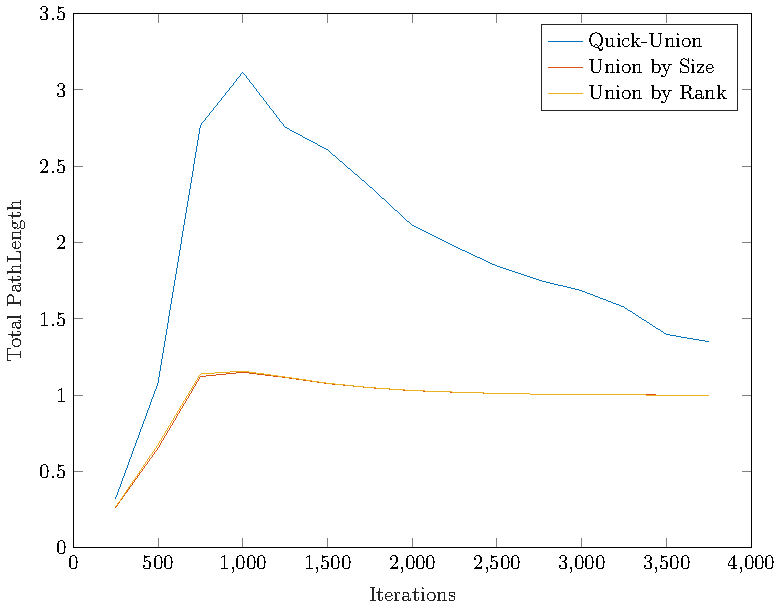
\includegraphics[width=\textwidth]{../images/plotPSFull1000_PathLength.pdf}
        \caption{Path Lengths with different union strategies with $n = 1000$ using Path Splitting}
    \end{subfigure}%
    \hfill
    % Subfigure 2
    \begin{subfigure}{0.32\textwidth}
        \centering
        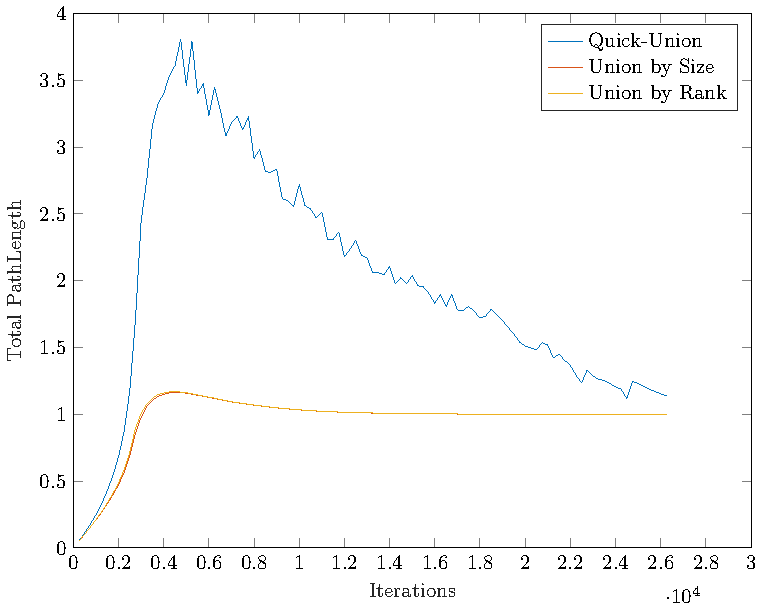
\includegraphics[width=\textwidth]{../images/plotPSFull5000_PathLength.pdf}
        \caption{Path Lengths with different union strategies with $n = 5000$ using Path Splitting}
    \end{subfigure}%
    \hfill
    % Subfigure 3
    \begin{subfigure}{0.32\textwidth}
        \centering
        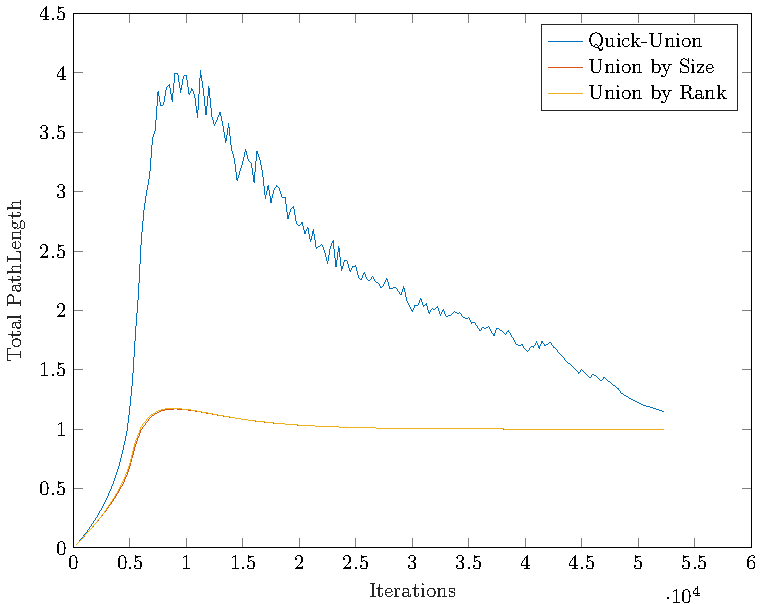
\includegraphics[width=\textwidth]{../images/plotPSFull10000_PathLength.pdf}
        \caption{Path Lengths with different union strategies with $n = 10000$ using Path Splitting}
    \end{subfigure}

    \begin{subfigure}{0.32\textwidth}
        \centering
        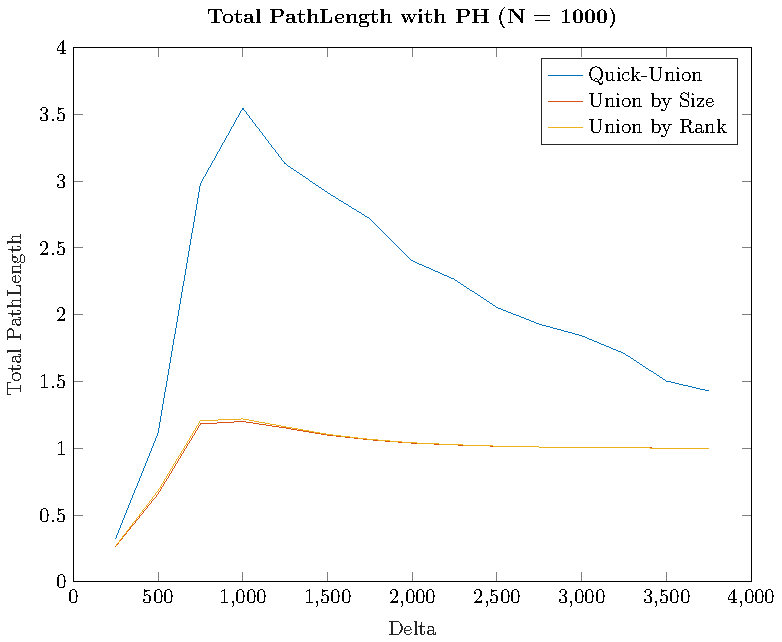
\includegraphics[width=\textwidth]{../images/plotPHFull1000_PathLength.pdf}
        \caption{Path Lengths with different union strategies with $n = 1000$ using Path Halving}
    \end{subfigure}%
    \hfill
    % Subfigure 2
    \begin{subfigure}{0.32\textwidth}
        \centering
        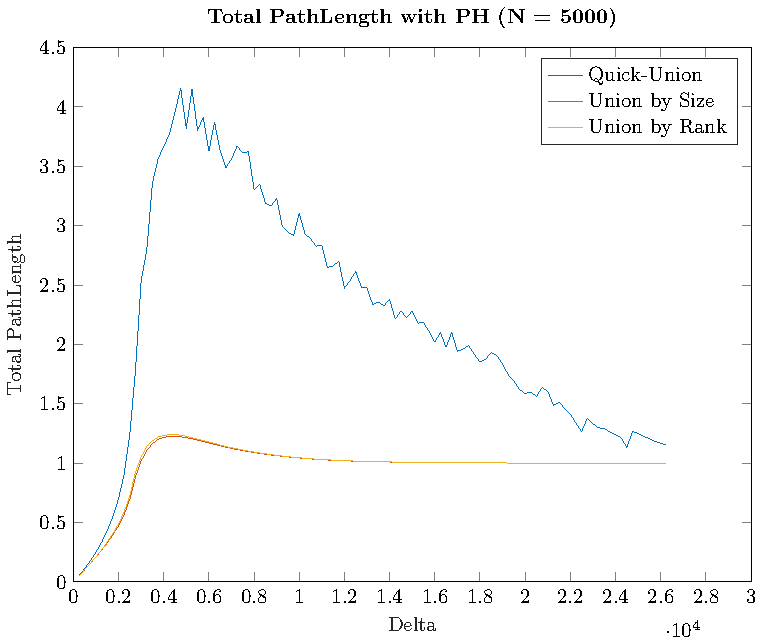
\includegraphics[width=\textwidth]{../images/plotPHFull5000_PathLength.pdf}
        \caption{Path Lengths with different union strategies with $n = 5000$ using Path Halving}
    \end{subfigure}%
    \hfill
    % Subfigure 3
    \begin{subfigure}{0.32\textwidth}
        \centering
        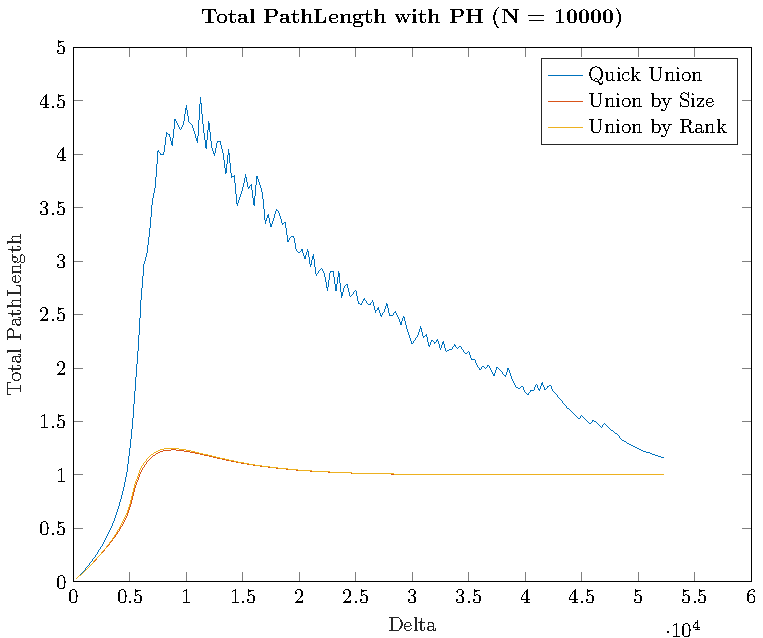
\includegraphics[width=\textwidth]{../images/plotPHFull10000_PathLength.pdf}
        \caption{Path Lengths with different union strategies with $n = 10000$ using Path Halving}
    \end{subfigure}

    \begin{subfigure}{0.32\textwidth}
        \centering
        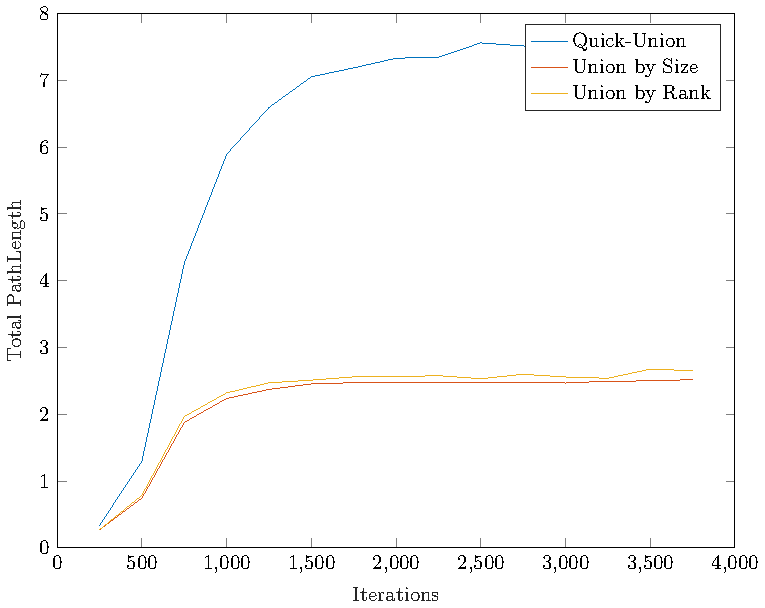
\includegraphics[width=\textwidth]{../images/plotTORFull1000_PathLength.pdf}
        \caption{Path Lengths with different union strategies with $n = 1000$ using Type One Reversal}
    \end{subfigure}%
    \hfill
    % Subfigure 2
    \begin{subfigure}{0.32\textwidth}
        \centering
        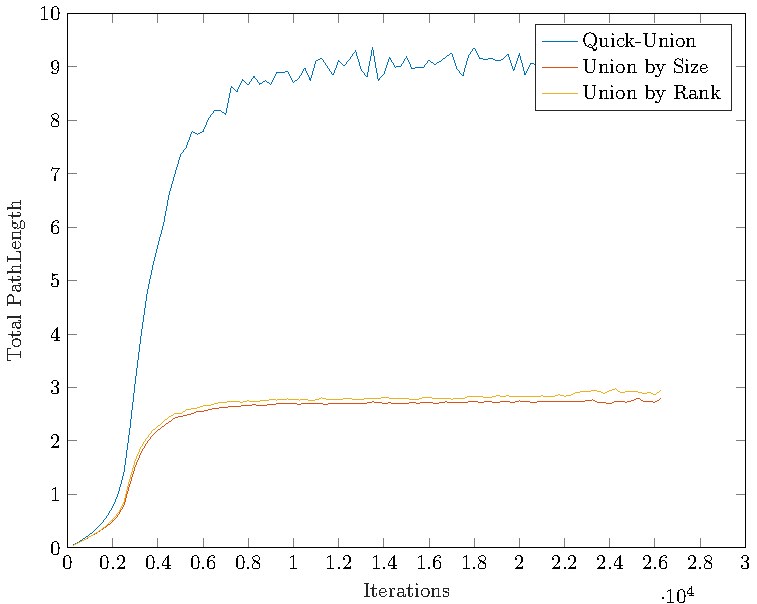
\includegraphics[width=\textwidth]{../images/plotTORFull5000_PathLength.pdf}
        \caption{Path Lengths with different union strategies with $n = 5000$ using Type One Reversal}
    \end{subfigure}%
    \hfill
    % Subfigure 3
    \begin{subfigure}{0.32\textwidth}
        \centering
        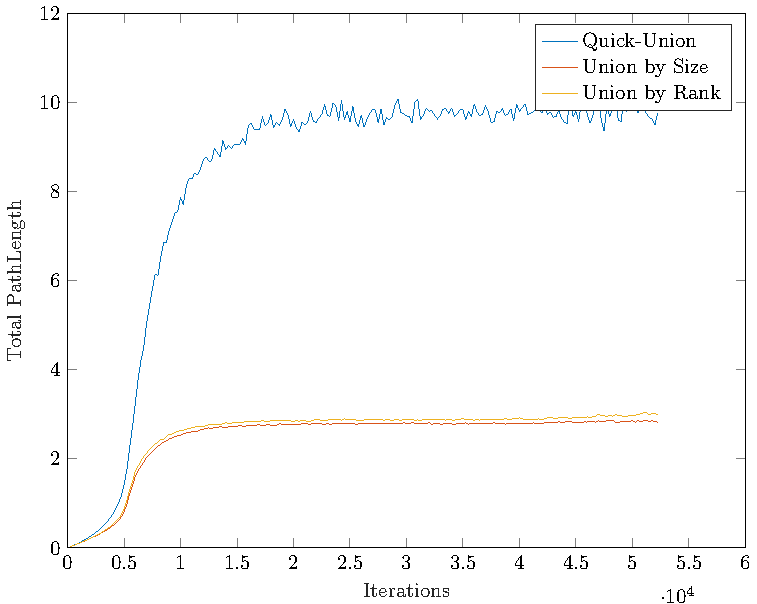
\includegraphics[width=\textwidth]{../images/plotTORFull10000_PathLength.pdf}
        \caption{Path Lengths with different union strategies with $n = 10000$ using Type One Reversal}
    \end{subfigure}

    \caption{Total Path Length normalized for different heuristics}
    \label{fig:tplH}
\end{figure}

\begin{figure}[ht]
    \centering
    \begin{subfigure}{0.32\textwidth}
        \centering
        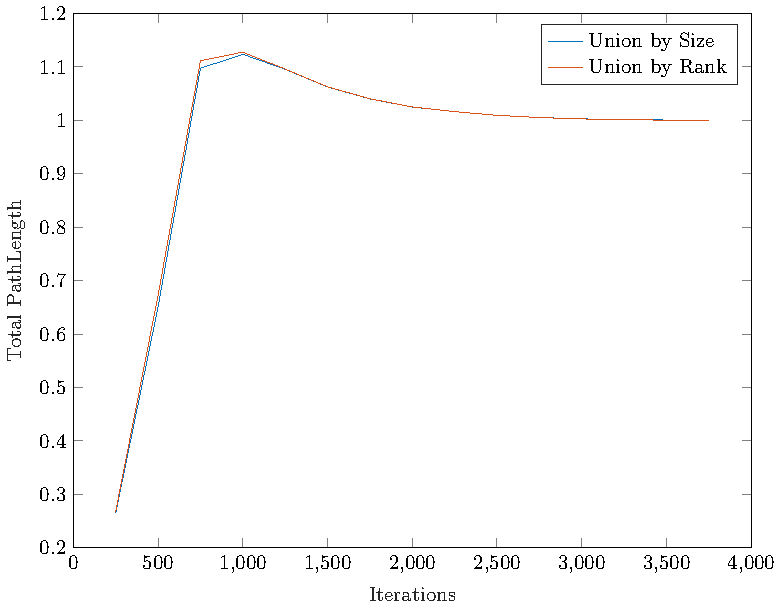
\includegraphics[width=\textwidth]{../images/plotFCNonFull1000_PathLength.pdf}
        \caption{Path Lengths with different union strategies with $n = 1000$ using Full Compression}
    \end{subfigure}%
    \hfill
    % Subfigure 2
    \begin{subfigure}{0.32\textwidth}
        \centering
        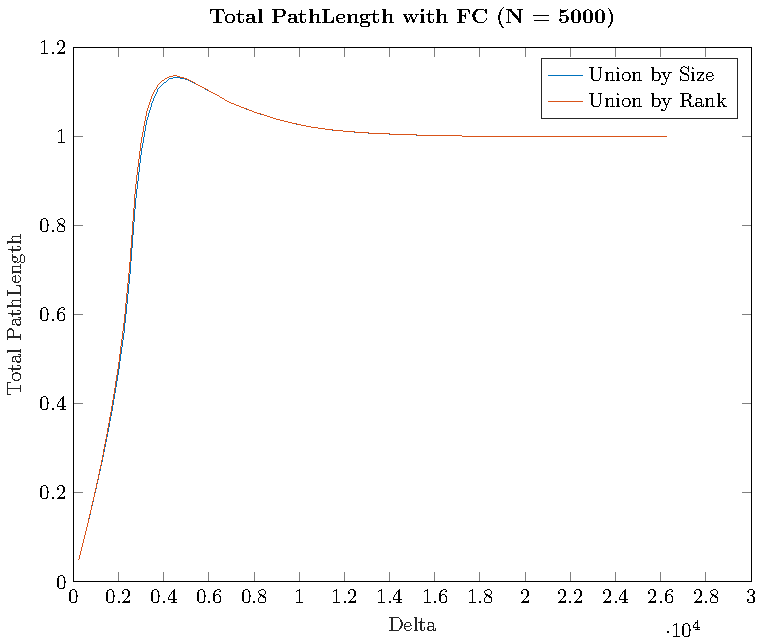
\includegraphics[width=\textwidth]{../images/plotFCNonFull5000_PathLength.pdf}
        \caption{Path Lengths with different union strategies with $n = 5000$ using Full Compression}
    \end{subfigure}%
    \hfill
    % Subfigure 3
    \begin{subfigure}{0.32\textwidth}
        \centering
        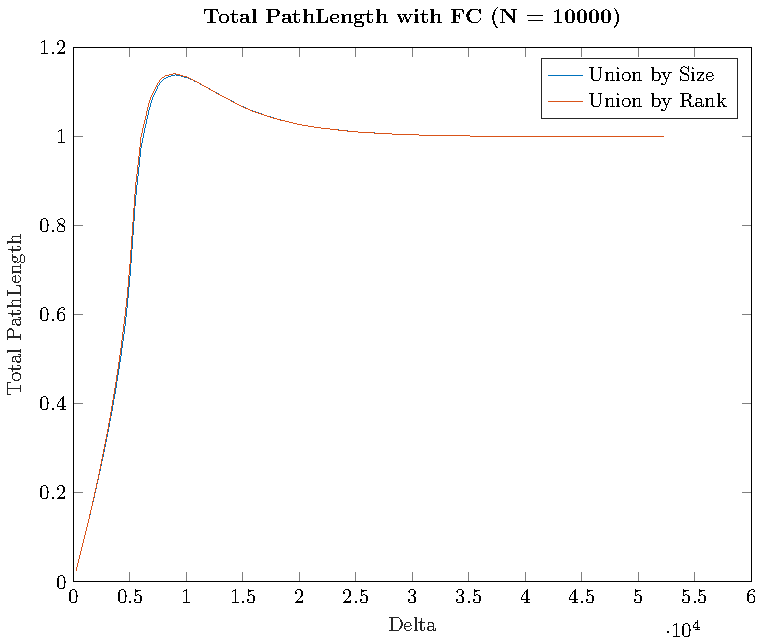
\includegraphics[width=\textwidth]{../images/plotFCNonFull10000_PathLength.pdf}
        \caption{Path Lengths with different union strategies with $n = 10000$ using Full Compression}
    \end{subfigure}
    % Subfigure 1
    \begin{subfigure}{0.32\textwidth}
        \centering
        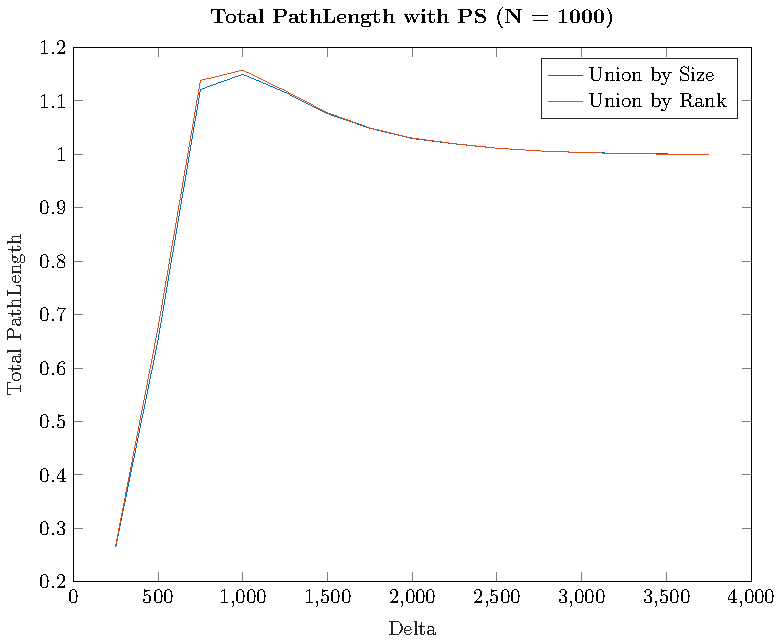
\includegraphics[width=\textwidth]{../images/plotPSNonFull1000_PathLength.pdf}
        \caption{Path Lengths with different union strategies with $n = 1000$ using Path Splitting}
    \end{subfigure}%
    \hfill
    % Subfigure 2
    \begin{subfigure}{0.32\textwidth}
        \centering
        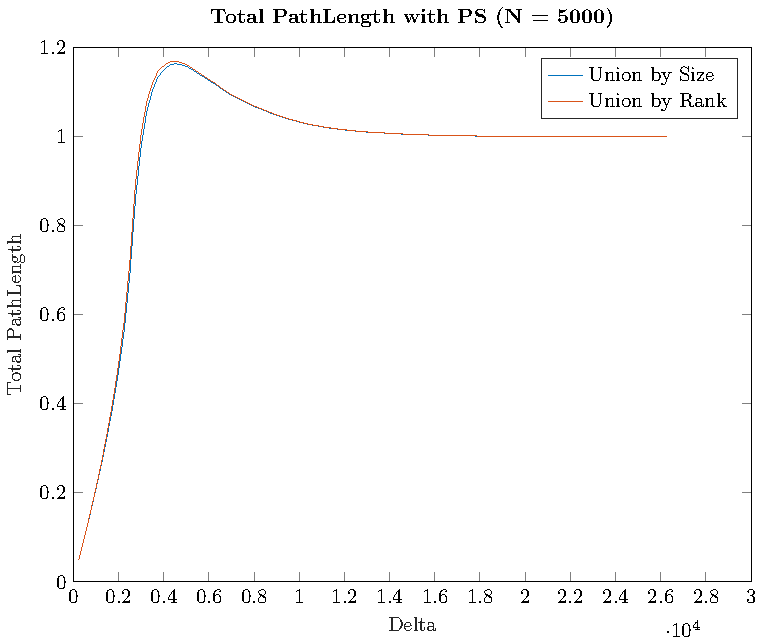
\includegraphics[width=\textwidth]{../images/plotPSNonFull5000_PathLength.pdf}
        \caption{Path Lengths with different union strategies with $n = 5000$ using Path Splitting}
    \end{subfigure}%
    \hfill
    % Subfigure 3
    \begin{subfigure}{0.32\textwidth}
        \centering
        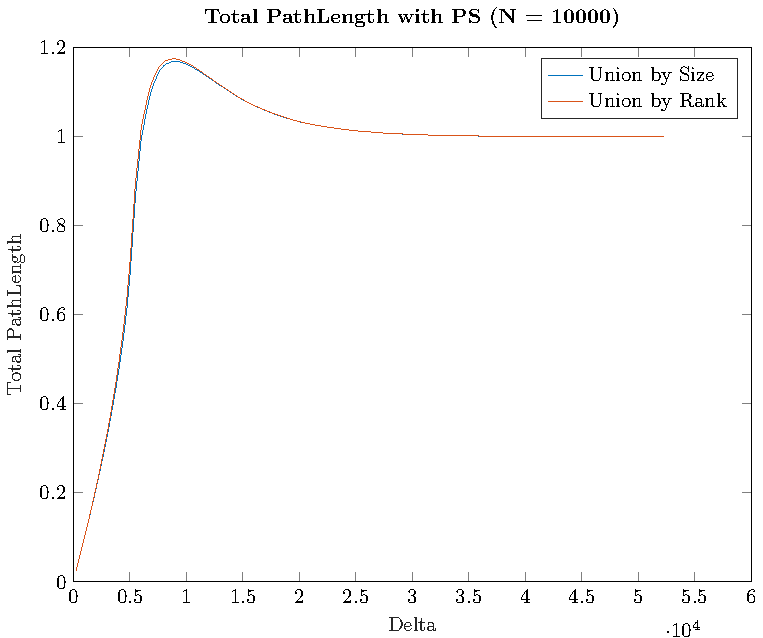
\includegraphics[width=\textwidth]{../images/plotPSNonFull10000_PathLength.pdf}
        \caption{Path Lengths with different union strategies with $n = 10000$ using Path Splitting}
    \end{subfigure}

    \begin{subfigure}{0.32\textwidth}
        \centering
        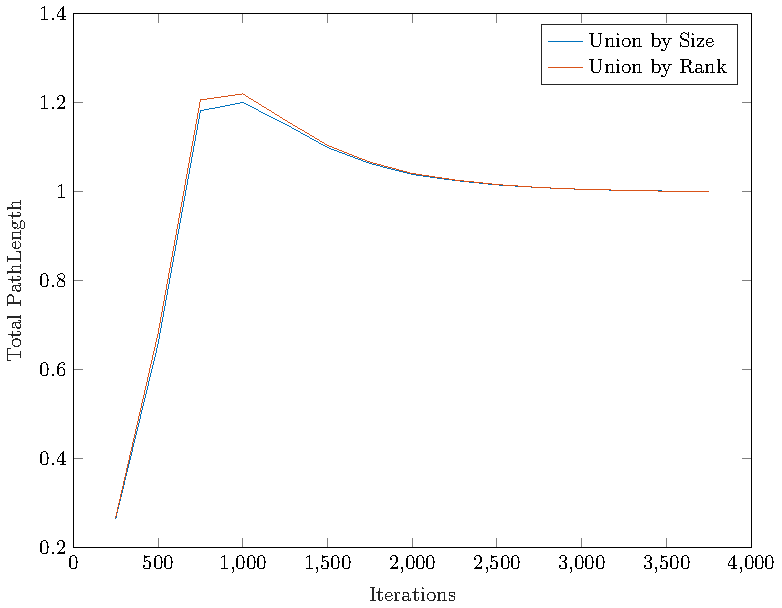
\includegraphics[width=\textwidth]{../images/plotPHNonFull1000_PathLength.pdf}
        \caption{Path Lengths with different union strategies with $n = 1000$ using Path Halving}
    \end{subfigure}%
    \hfill
    % Subfigure 2
    \begin{subfigure}{0.32\textwidth}
        \centering
        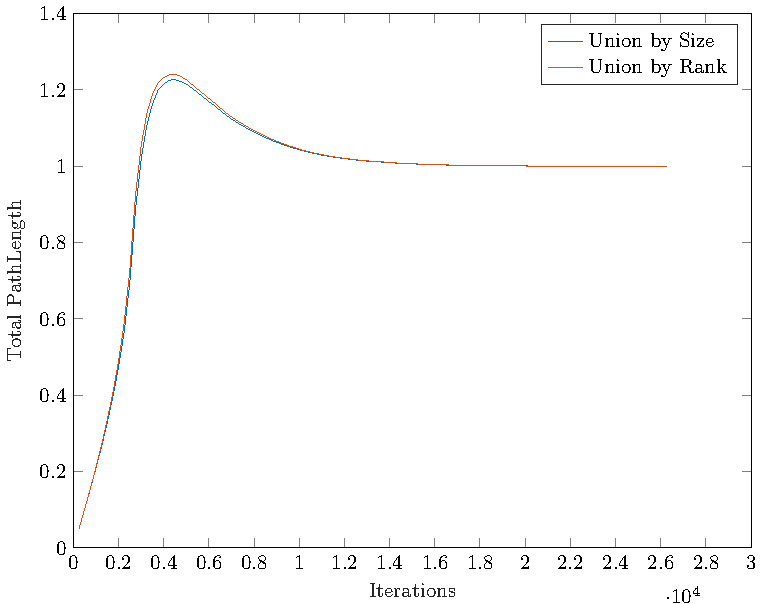
\includegraphics[width=\textwidth]{../images/plotPHNonFull5000_PathLength.pdf}
        \caption{Path Lengths with different union strategies with $n = 5000$ using Path Halving}
    \end{subfigure}%
    \hfill
    % Subfigure 3
    \begin{subfigure}{0.32\textwidth}
        \centering
        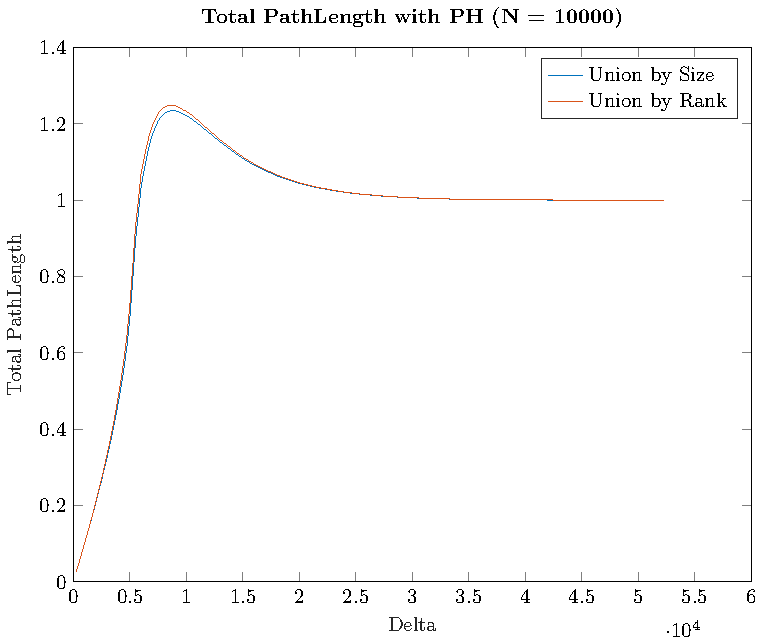
\includegraphics[width=\textwidth]{../images/plotPHNonFull10000_PathLength.pdf}
        \caption{Path Lengths with different union strategies with $n = 10000$ using Path Halving}
    \end{subfigure}
    \begin{subfigure}{0.32\textwidth}
        \centering
        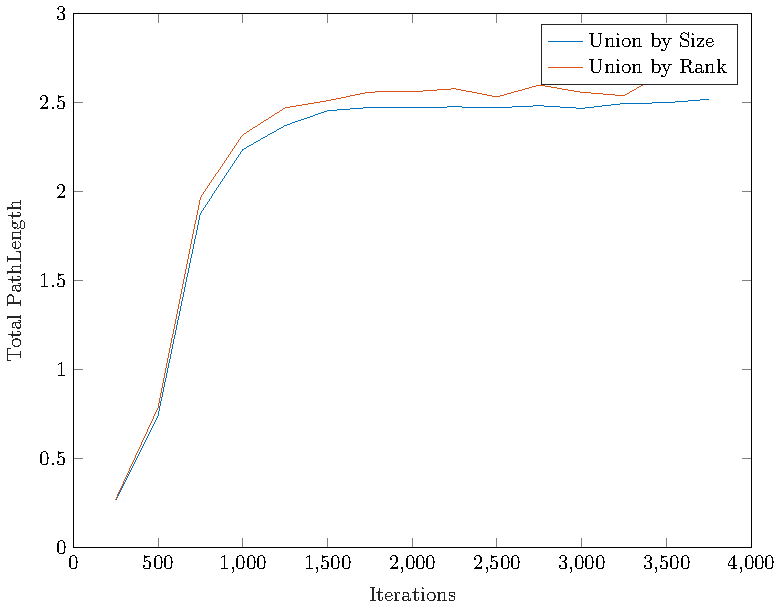
\includegraphics[width=\textwidth]{../images/plotTORNonFull1000_PathLength.pdf}
        \caption{Path Lengths with different union strategies with $n = 1000$ using Type One Reversal}
    \end{subfigure}%
    \hfill
    % Subfigure 2
    \begin{subfigure}{0.32\textwidth}
        \centering
        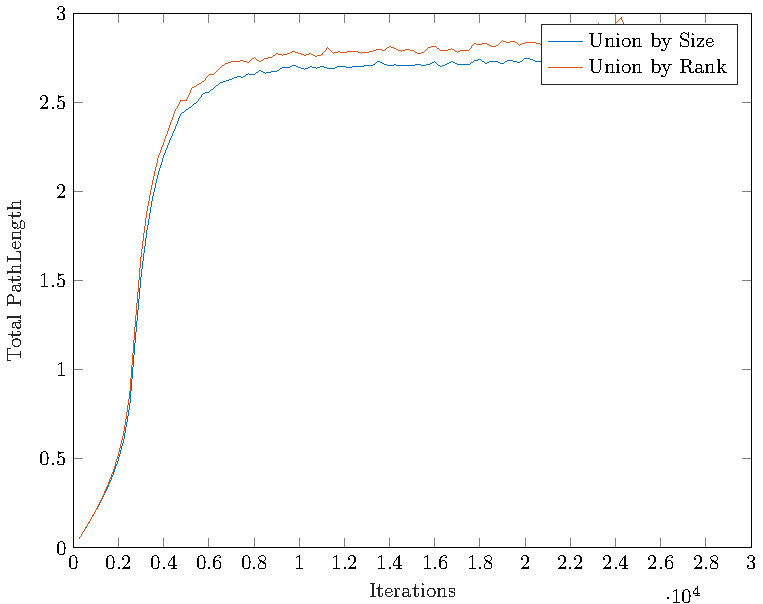
\includegraphics[width=\textwidth]{../images/plotTORNonFull5000_PathLength.pdf}
        \caption{Path Lengths with different union strategies with $n = 5000$ using Type One Reversal}
    \end{subfigure}%
    \hfill
    % Subfigure 3
    \begin{subfigure}{0.32\textwidth}
        \centering
        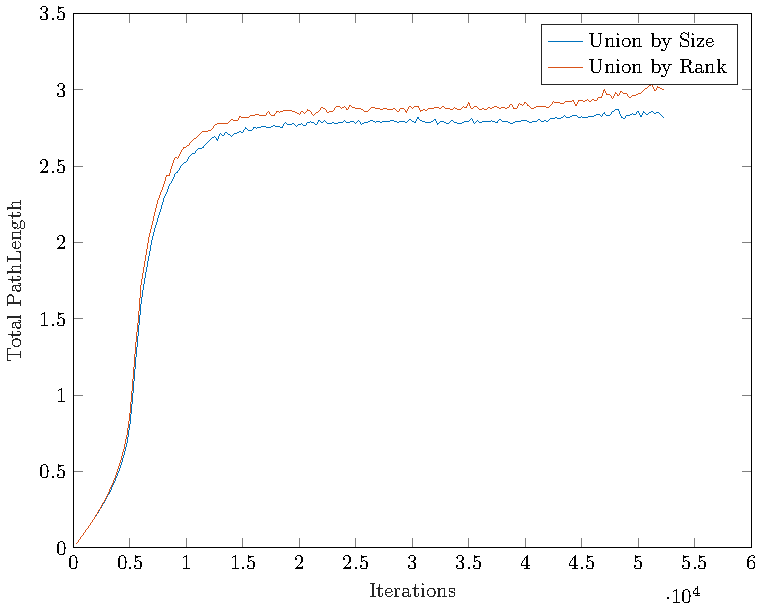
\includegraphics[width=\textwidth]{../images/plotTORNonFull10000_PathLength.pdf}
        \caption{Path Lengths with different union strategies with $n = 10000$ using Type One Reversal}
    \end{subfigure}

    \caption{Total Path Length normalized for different heuristics without Quick-Union}
    \label{fig:tplNH}
\end{figure}
